% This is "sig-alternate.tex" V2.0 May 2012
% This file should be compiled with V2.5 of "sig-alternate.cls" May 2012
%
% This example file demonstrates the use of the 'sig-alternate.cls'
% V2.5 LaTeX2e document class file. It is for those submitting
% articles to ACM Conference Proceedings WHO DO NOT WISH TO
% STRICTLY ADHERE TO THE SIGS (PUBS-BOARD-ENDORSED) STYLE.
% The 'sig-alternate.cls' file will produce a similar-looking,
% albeit, 'tighter' paper resulting in, invariably, fewer pages.
%
% ----------------------------------------------------------------------------------------------------------------
% This .tex file (and associated .cls V2.5) produces:
%       1) The Permission Statement
%       2) The Conference (location) Info information
%       3) The Copyright Line with ACM data
%       4) NO page numbers
%
% as against the acm_proc_article-sp.cls file which
% DOES NOT produce 1) thru' 3) above.
%
% Using 'sig-alternate.cls' you have control, however, from within
% the source .tex file, over both the CopyrightYear
% (defaulted to 200X) and the ACM Copyright Data
% (defaulted to X-XXXXX-XX-X/XX/XX).
% e.g.
% \CopyrightYear{2007} will cause 2007 to appear in the copyright line.
% \crdata{0-12345-67-8/90/12} will cause 0-12345-67-8/90/12 to appear in the copyright line.
%
% ---------------------------------------------------------------------------------------------------------------
% This .tex source is an example which *does* use
% the .bib file (from which the .bbl file % is produced).
% REMEMBER HOWEVER: After having produced the .bbl file,
% and prior to final submission, you *NEED* to 'insert'
% your .bbl file into your source .tex file so as to provide
% ONE 'self-contained' source file.
%
% ================= IF YOU HAVE QUESTIONS =======================
% Questions regarding the SIGS styles, SIGS policies and
% procedures, Conferences etc. should be sent to
% Adrienne Griscti (griscti@acm.org)
%
% Technical questions _only_ to
% Gerald Murray (murray@hq.acm.org)
% ===============================================================
%
% For tracking purposes - this is V2.0 - May 2012

\documentclass{sig-alternate}
\usepackage{adjustbox}
\usepackage{graphicx}
\usepackage{multirow}
\usepackage{pdflscape}
\usepackage{subcaption}
\usepackage{url}
\usepackage[numbers]{natbib}
\newcommand{\citenoun}[1]{{\citeauthor{#1}~\cite{#1}}}

\begin{document}
%
% --- Author Metadata here ---
%\conferenceinfo{WOODSTOCK}{'97 El Paso, Texas USA}
%\CopyrightYear{2007} % Allows default copyright year (20XX) to be over-ridden - IF NEED BE.
%\crdata{0-12345-67-8/90/01}  % Allows default copyright data (0-89791-88-6/97/05) to be over-ridden - IF NEED BE.
% --- End of Author Metadata ---

\title{A demographic and sentiment analysis of e-cigarette messages on Twitter}
%
% You need the command \numberofauthors to handle the 'placement
% and alignment' of the authors beneath the title.
%
% For aesthetic reasons, we recommend 'three authors at a time'
% i.e. three 'name/affiliation blocks' be placed beneath the title.
%
% NOTE: You are NOT restricted in how many 'rows' of
% "name/affiliations" may appear. We just ask that you restrict
% the number of 'columns' to three.
%
% Because of the available 'opening page real-estate'
% we ask you to refrain from putting more than six authors
% (two rows with three columns) beneath the article title.
% More than six makes the first-page appear very cluttered indeed.
%
% Use the \alignauthor commands to handle the names
% and affiliations for an 'aesthetic maximum' of six authors.
% Add names, affiliations, addresses for
% the seventh etc. author(s) as the argument for the
% \additionalauthors command.
% These 'additional authors' will be output/set for you
% without further effort on your part as the last section in
% the body of your article BEFORE References or any Appendices.

\numberofauthors{1} %  in this sample file, there are a *total*
% of EIGHT authors. SIX appear on the 'first-page' (for formatting
% reasons) and the remaining two appear in the \additionalauthors section.
%
\author{
% You can go ahead and credit any number of authors here,
% e.g. one 'row of three' or two rows (consisting of one row of three
% and a second row of one, two or three).
%
% The command \alignauthor (no curly braces needed) should
% precede each author name, affiliation/snail-mail address and
% e-mail address. Additionally, tag each line of
% affiliation/address with \affaddr, and tag the
% e-mail address with \email.
%
% 1st. author
\alignauthor
Elaine Cristina Resende and Aron Culotta\\
       \affaddr{Department of Computer Science}\\
       \affaddr{Illinois Institute of Technology}\\
       \affaddr{Chicago, IL}\\
       \email{eresende@hawk.iit.edu, culotta@cs.iit.edu}
}
% There's nothing stopping you putting the seventh, eighth, etc.
% author on the opening page (as the 'third row') but we ask,
% for aesthetic reasons that you place these 'additional authors'
% in the \additional authors block, viz.
%\additionalauthors{Additional authors: John Smith (The Th{\o}rv{\"a}ld Group,
%email: {\texttt{jsmith@affiliation.org}}) and Julius P.~Kumquat
%(The Kumquat Consortium, email: {\texttt{jpkumquat@consortium.net}}).}
%\date{30 July 1999}
% Just remember to make sure that the TOTAL number of authors
% is the number that will appear on the first page PLUS the
% number that will appear in the \additionalauthors section.

\maketitle
\begin{abstract}
Social media provide a potentially useful new data source to understand emerging public health behaviors. In this paper, we study messages about e-cigarettes posted to Twitter.com. We apply methods to classify messages by sentiment and to estimate the gender and age of users. We apply our approach to nearly one million messages about e-cigarettes posted from October 2012 to September 2013. We find that overall volume of e-cigarette tweets increased five-fold (from 30K per month to 150K per month); and that males and younger users were more likely to post positive messages about e-cigarettes. A qualitative analysis also reveals several trends, such as negative sentiment toward people who smoke in class; females giving e-cigarettes to relatives to help them quit smoking; and spikes in people using e-cigarettes to quit smoking in January.
\end{abstract}

% A category with the (minimum) three required fields
\category{I.5.4}{Pattern Recognition}{Applications--Text processing}
\category{H.4}{Information Systems Applications}{Miscellaneous}
%A category including the fourth, optional field follows...
%\category{D.2.8}{Software Engineering}{Metrics}[complexity measures, performance measures]

\keywords{Web mining, social media, public health}

\begin{table*}[ht!]
\centering
\caption{Training Data Summary\label{tab:labelsample}}
\begin{tabular}{|l|l|p{9cm}|}
\hline
{\bf Class}                     & {\bf \#Tweets}        & {\bf Tweet Sample}                                                                                                                       \\ \hline
\multirow{2}{*}{{\bf Positive}} & \multirow{2}{*}{707}  & I bought a Ecig today                                                                                                                    \\ %\cline{3-3} 
                                &                       & Electric cigarettes are better than regular cigarettes!!                                          \\ \hline
\multirow{2}{*}{{\bf Negative}} & \multirow{2}{*}{279}  & \#IHatePeopleThat smoke ecigs                                                  \\ %\cline{3-3} 
                                &                       & e-cigs are bad, mmkay?                                                                                                         \\ \hline
\multirow{2}{*}{{\bf Neutral}}  & \multirow{2}{*}{1014} &  what is an electronic cigarette?        \\ % \cline{3-3} 
                                &                       & A homeless guy just asked me if he could bum an e-cigarette\\ \hline
\end{tabular}
\end{table*}



\section{Introduction}
Understanding evolving behaviors and attitudes related to alcohol, tobacco,
and other drugs is a critical public health goal. Typically, such topics are
investigated by survey research; however, surveys can be costly and
time-consuming, making them ill-suited to rapidly changing
environments. Furthermore, survey response rates have fallen precipitously in
recent years (Kohut et al. 2012), leading researchers to seek non-traditional
data sources. A promising new methodology is social media analysis, which
analyzes online content expressing health-related behaviors and opinions to
provide insights into population-level trends. Online content offers several
potential advantages over traditional data: one can in real-time measure how
behaviors and attitudes change in response to rare events such as legal
changes, new products, and marketing campaigns, and the open-ended nature of
the content can provide more diverse data. Such approaches have been used to
study depression~\cite{choudhury2013predicting}, insomnia~\cite{powell2012i},
and other health topics~\cite{dredze2012how}.

In this paper we present a descriptive study of attitudes towards electronic
cigarettes (e-cigs) expressed on Twitter. E-cigs provide a
nicotine-containing aerosol with different flavors, glycol and other
ingredients that users smoke by heating up a solution
\cite{grana2014cigarettes}. E-cig adoption has increased rapidly in the United
States recently~\cite{king2013awareness,centers2013notes}; by one estimate,
usage by high school students tripled in 2014~\cite{ecig2015triples}. Despite
this rapid growth, there is still considerable debate over the health impact
of e-cigs~\cite{sussan2015exposure,pauly2007tobacco,bhatnagar2014electronic},
also reflected in consumer surveys~\cite{pepper2015risky}, leading to
uncertainty as to how they should be regulated.

We analyze nearly one million tweets posted from October 2012 to September
2013 that contain keywords related to e-cigarettes. We use a supervised
classification algorithm to annotate each message by sentiment (positive,
negative, or neutral). Additionally, using the first name of each user, we
derive estimates of age and gender to further stratify results. Our main
findings are as follows:
\begin{itemize}
\item Overall volume of e-cig tweets grew five-fold in our year sample, from
  30K tweets in October 2012 to 150K in September 2013.
\item Of tweets expressing sentiment, 65\% are classified as positive
  sentiment (tweets either advocating for e-cigs or indicating that the user
  has tried e-cigs). This value ranges by month from 61\% in March 2013 to
  74\% in July 2013. 
\item We find positive sentiment to be slightly higher for males than females
  (63\% vs.~61\%), and highest for users estimated to be 18-24 years old (67\%).
\end{itemize}

We additionally perform a qualitative analysis to provide a more fine-grained
insight into the different ways people discuss e-cigs and how that is related
to sentiment and demographics. For example, in November-January we find a
spike in messages from users wishing for e-cigs as a Christmas present to help
them stop smoking. We also find that many tweets from young female users
mention smoking e-cigs with their parents or buying e-cigs for their parents;
whereas male users are more likely to ridicule those using e-cigs.

The remainder of the paper is organized as follows: Section~\ref{s.prior}
reviews related work; Section~\ref{s.methods} describes the Twitter data and
our method of analysis; Section~\ref{s.results} describes our main results;
Section~\ref{s.conclusion} discusses implications, limitations, and future
work.



\section{Prior work}
\label{s.prior}

\citenoun{myslin2013using} manually classified 4K tobacco-related tweets
along 30 dimensions, including sentiment, theme, and genre, finding that
tweets about e-cigs and hookahs tended to have more positive sentiment. Here,
we focus specifically on e-cigs, expanding upon this initial work with a much
larger set of tweets (1M) over a longer time span, and further
stratifying by gender and age.

\citenoun{huang2014cross} analyzed 74K tweets related to e-cigs and,
using a supervised classifier, found that 90\% were commercial tweets, and
about 10\% mentioned smoking cessation. We build on this prior work, using
their classifier to first filter out commercial tweets.

Other work has found a prevalence of smoking cessation accounts on
Twitter~\cite{prochaska2012twitter}, and has attempted to track the progress
of cessation attempts by following Twitter accounts of identified
users~\cite{murnane2014unraveling}.

Very recently, \citenoun{godea2015analysis} analyzed 106K tweets containing
e-cig related terms collected over a two month period. They built a sentiment
classifier using a hand-engineered lexicon of over 600 terms, achieving a
positive/negative F1-score of 55-56\%.

Compared to this prior work, our main contributions consist of (1) an analysis
of a much larger sample of e-cig tweets than has been done previously,
consisting of nearly one million tweets written over one year; (2) a sentiment
classifier tuned for precision that identifies positive tweets with 96\%
precision and negative tweets with 70\% precision; (3) an analysis of temporal
trends in sentiment and demographics.

\section{Methods}
\label{s.methods}

In this section we describe the data collected and the methods used for classifying messages by sentiment, age, and gender.


\subsection{Data Collection}
\label{sec:data}
We use the data collection process described in
\citenoun{huang2014cross}. Using the full Twitter Firehose, tweets were
collected from October 2012 to September 2013 using a set of keywords
identified by expert consensus ({\it e-cigarette}, {\it ecigarette}, {\it
  e-cig}, {\it ecig}). Additional tweets were identified that matched the
query: ({\it cig} OR {\it cigarette}) AND ({\it electronic} OR {\it blu} OR
{\it njoy}) (the latter two terms referring to the top-selling e-cig brands in
the U.S.). This resulted in 4,639,885 tweets. Using the classifier of
\citenoun{huang2014cross}, we retained only those tweets identified as
``organic,'' defined as ``those reflecting individual opinions or experiences
or linked to non-promotional content.'' This left 992,633 tweets.

On Twitter it is common for very similar messages to be posted many times,
either as retweets or as part of a coordinated marketing
campaign. Additionally, a number of accounts in our data are primarily focused
on e-cigarettes, either as an official corporate account, or as ``astroturf'' accounts that are created to artificially inflate the perceived
sentiment towards e-cigs~\cite{ratkiewicz2011truthy}.  As we are primarily
interested in the sentiment of genuine, ordinary users, we further filtered
the data as follows: (1) we removed all retweets; (2) we removed all tweets
whose content was duplicated in other tweets; (3) we retained only the first
tweet from each user. Figure~\ref{f.total} shows the number of tweets per
month for each filtering step. After all filtering, 455,648 tweets remain.


\subsection{Sentiment Classification}

We next wished to classify each tweet by sentiment towards e-cigs. To do so, we fit a supervised classifier (logistic regression) to a collection of manually annotated tweets. From the 455K tweets above, we uniformly sampled 2,000 tweets and manually categorized them as positive, negative or neutral as follows: 
\begin{itemize}
\item  tweets from users who expressed buying or use desire, or from users who tweeted about their e-cigs, or who expressed support of e-cigs were labeled as {\bf positive}; 
\item  tweets from users who were expressing complaints or antipathy towards e-cigs were labeled as {\bf negative}. 
\item  tweets from merchandising companies, news about electronic cigarettes, and tweets belonging to other languages were labeled as {\bf neutral}; they did not express any sentiment.
\end{itemize}

Note that our definition of {\bf positive} is a bit different from typical sentiment classification; by including tweets indicating possible usage of e-cigs, we hoped to capture general notions of popularity of e-cigs, as opposed to simply opinions about e-cigs.

\begin{table*}[t]
\centering
\caption{Top Coefficients of Classifier\label{t.coef}}
\begin{tabular}{|r|p{14cm}| }
\hline
{\bf negative} & you, smoking, smoking an, he, fuck, people, smokes, an, faggot, are, class, smoke, stupid, in, look, shit, her, pussy, sorry, one\\
\hline
{\bf neutral} & URL, e-cigarettes, de, la, 99, retail, URL retail, ni, e-cigarette, markten, store, by, cigarette, of, dallas, smokers, 9999, @vaper\_trail, electronic, may\\
\hline
{\bf positive} & my, i, vaping, \#vaping, \#ecig, my ecig, me, we, \#vape, got, e-cig, my e-cig, \#euecigban, my e, vape, i'm, good, this, i need, to black\\
\hline

\end{tabular}
\end{table*}


Table \ref{tab:labelsample} describes some examples of our training data with tweets, their classes and also the distribution of each class. We can see that roughly 51\% of the tweets were labeled as neutral, 14\% as negative and 35\% as positive. 

We fit a logistic regression classifier to the labeled tweets, using L2 regularization. After a series of pilot experiments, we adopted the following tokenization scheme: (1) convert to lower case; (2) maintain hashtags and mention terms; (3) remove punctuation (except for internal punctuation like hyphens and apostrophes); (4) remove characters repeated more than twice consecutively; (5) collapse all URLs to the same term; (6) collapse all digits to the same character. We retain both unigrams and bigrams, removing any term that does not occur in at least two tweets. We represent each tweet by a tf-idf vector (dividing term frequency by document frequency), normalized to unit length.\footnote{All code to reproduce our analysis is available at \url{https://github.com/tapilab/chs-2015-ecig}.}

Figure~\ref{f.prec_rec} displays the precision-recall curves for the logistic regression classifier using 10-fold cross-validation on the 2,000 hand-labeled tweets; Table~\ref{t.measure} reports the precision, recall, and F1 metrics for each class; and Table~\ref{t.coef} reports the top-weighted coefficients per class.

\begin{figure}[t]
\caption{Precision-recall curves derived by classifying the labeled data using 10-fold cross-validation.}
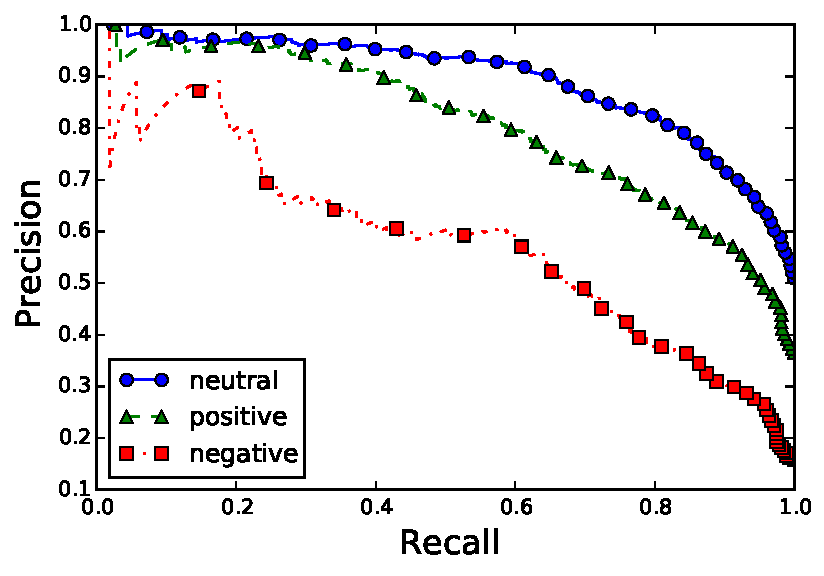
\includegraphics[width=\columnwidth]{nb/prec_rec.pdf}  % 111.png}
\centering
\label{f.prec_rec}
\end{figure}

\begin{table}[t]
\caption{Cross-validation classification accuracy \label{t.measure}}
\centering
\begin{tabular}{|r|c|c|c|c|}
\hline
 & {\bf Prec} & {\bf Rec} & {\bf F1} & {\bf N}\\
\hline
{\bf negative} & 0.84 & 0.83 & 0.84 & 1296\\
{\bf positive} & 0.70 & 0.72 & 0.71 & 704\\
\hline
{\bf avg} & 0.79 & 0.79 & 0.79 & 2000\\
\hline
\end{tabular}
\end{table}




The F1 score averaged over each class is .74; the classifier is most accurate on the neutral class (.81 F1) and least accurate on the negative class (.57 F1).

Table~\ref{t.coef} suggests that negative tweets are mostly ridiculing other people who use e-cigs, while positive tweets are typically first-person accounts of wanting or using e-cigs. Many of the neutral tweets are marketing related (that were missed by prior filters) or informative, as indicated by the presence of links, typically to news stories.

While the classifier accuracy is higher than that reported in prior work on a
related task (\citenoun{godea2015analysis} report F1 scores of 55-56\% for
positive/negative classes), we desire a high precision classifier to
strengthen the validity of the conclusions drawn from its application to the
remaining unlabeled tweets. Fortunately, we can use confidence thresholds to
improve the precision. The precision-recall graph indicates that if we
restrict our classifications to the 25\% that the classifier is most confident
in, the precision values for the positive and negative classes are .96 and
.70, respectively. To classify each of the 455K unlabeled tweets, then, we
apply the classifier trained on the 2,000 labeled tweets, setting confidence
thresholds to achieve these levels of precision (the confidence threshold is
.65 for the positive class and .5 for the negative class). Classifications
below these thresholds are placed in the neutral class. Thus, we reduce the
number of tweets labeled as sentiment-bearing, but increase the precision of
the remaining classifications.

\subsection{Gender and Age Inference}

Following the work of \citenoun{paval2015confounds} and
\citenoun{silver2014how}, we use name statistics to estimate the gender and
age of each user in the data. We extract the first token from the {\it name} field in the user's profile, where available. We then compare this to government statistics regarding the gender and age distribution for each name.

For gender, we collect names from the census that comprise 75\% of the
population (to remove rare names that may produce false matches, such as {\it
  The}). We additionally remove names that appear both as male and female
names. This results in 226 male and 518 female names. We use these two lists to assign each user a gender label, when possible.

For age, we use data from the Social Security Administration indicating baby names by year, along with life expectancy tables, to estimate the age distribution of a person with a given name. We define the years in age brackets (under 18, 18-24, 25-34, 35-44 and 45+). Thus, for each user with a matching name, we produce a probability distribution over the five age brackets. See \citenoun{silver2014how} for more details.

\section{Results}
\label{s.results}

Here we report results of sentiment, age, and gender inference.

\begin{figure*}[t]
  \caption{Tweets by month and sentiment.}
  \begin{subfigure}{.96\columnwidth}
    \centering
    \caption{Tweets by month. \label{f.total}}
    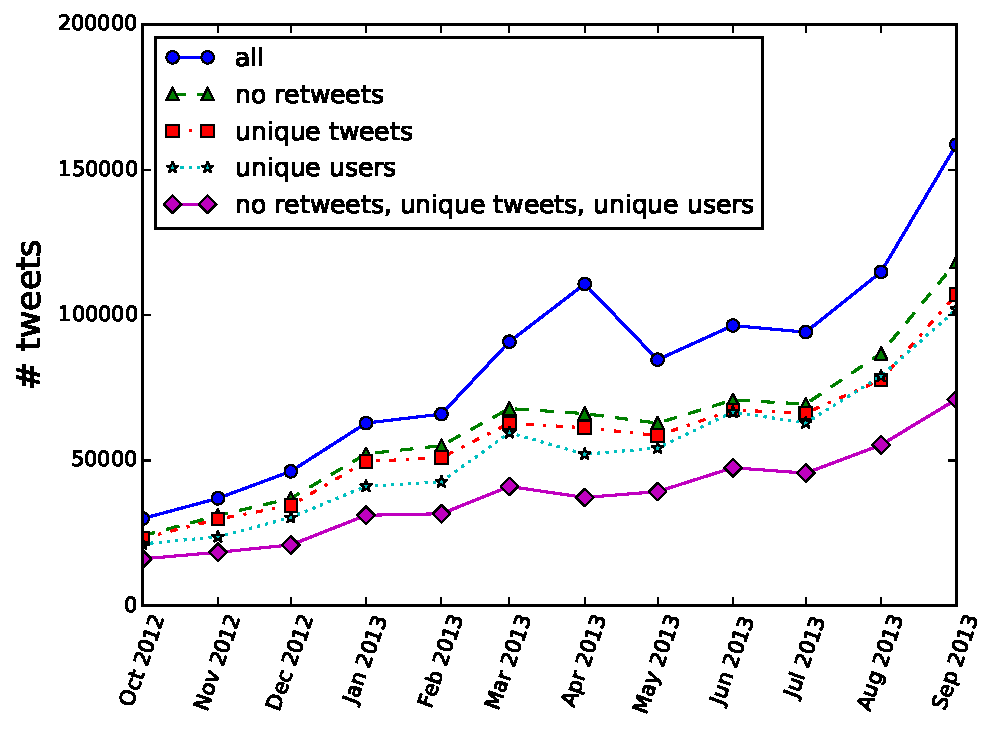
\includegraphics[width=\columnwidth]{nb/raw_counts.pdf}  % 111.png}
  \end{subfigure}
  \begin{subfigure}{\columnwidth}
    \centering
    \caption{Tweets by sentiment. \label{f.sentiment}}
    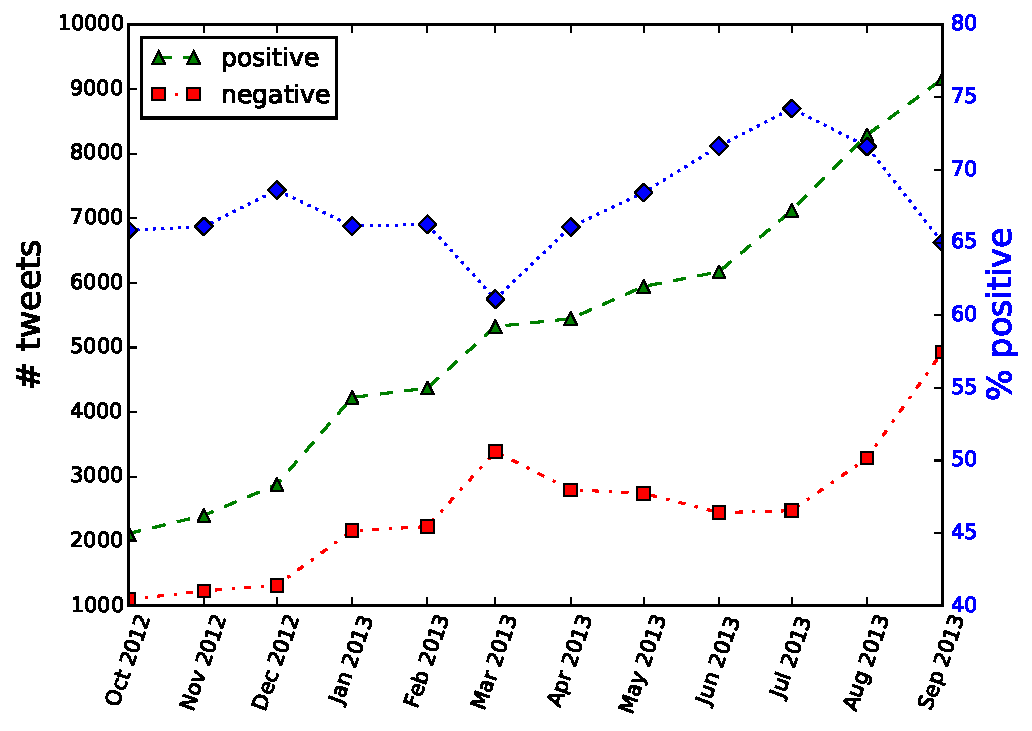
\includegraphics[width=\columnwidth]{nb/sentiment.pdf}
  \end{subfigure}
\end{figure*}

\begin{figure}[t]
  \caption{Percent of non-neutral tweets mentioning each term. \label{f.terms}}
  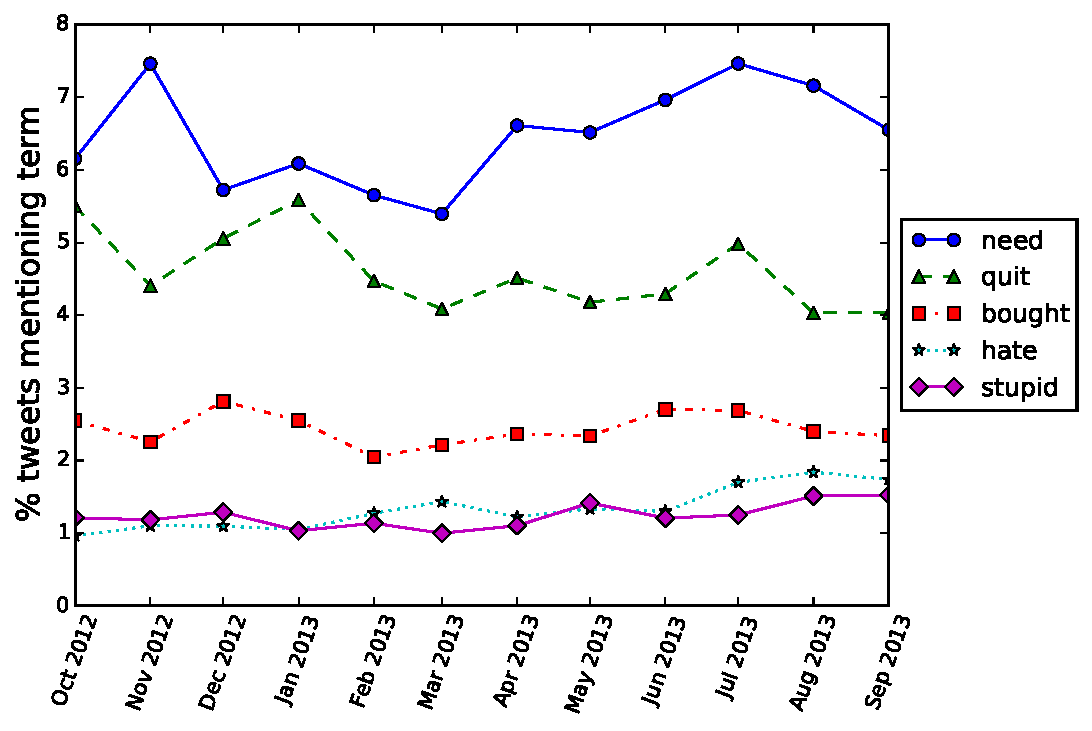
\includegraphics[width=\columnwidth]{nb/term_trends.pdf}  % 111.png}
\end{figure}

\subsection{Sentiment}
\label{s.sentiment_results}
The sentiment classifier returns 103,103 positive and 56,652 negative tweets
from the 455K unlabeled tweets. Figure~\ref{f.sentiment} plots the sentiment
per month. Additionally, in the second y-axis, we report the percentage of
non-neutral tweets that are labeled as positive (i.e.,
$\frac{\hbox{\#positive}}{\hbox{\#positive } + \hbox{ \#negative}}$). Overall,
65\% of the non-neutral tweets are labeled as positive. We emphasize that this
does not mean that 65\% of Twitter users like e-cigs; rather, when a Twitter
user posts a message about e-cigs, it is more likely to be in the positive
class (e.g., about using or wanting to use e-cigs) than in the negative class
(e.g., ridiculing the use of e-cigs).

There appears to be a mild increasing trend in percent of positive sentiment
during this time period (a linear fit yields a slope of .41), but there is an
obvious dip in March 2013 and spike in July 2013. In March, the South Korean
singer Onew was photographed smoking an e-cig. Due to his reputation as a role
model for his young fans, this news led to many critical tweets. Even after
our filtering steps to remove retweets and duplicate tweets, this still
resulted in 1,127 unique tweets mentioning Onew (out of 41K tweets in
March). Of these 1,127 tweets, 470 were classified as positive and 2 were
classified as negative. A representative negative tweet is: ``{\it He smokes
  too WTF ONEW WHYYY! Not a cig but an electronic one at that!}"

The spike in sentiment in July does not appear to be related to one event. There is a gradual increase from March through July, then a swift decline in August and September. We believe this is due in large part to a common type of negative tweet in which a student criticizes another student for smoking e-cigs in a classroom, e.g.,  ``{\it Who uses an e-cig during class? \#Idiot}.''

To further investigate this, Figure~\ref{f.terms} plots by month the percentage of all sentiment-bearing tweets containing a hand-selected set of keywords. For example, in November 2012, over 4\% of all tweets classified as positive or negative contained the term ``class.'' We can see that this plot closely matches the U.S. academic calendar, with drops in December, June, and July. There also appear to be spikes at the start of each school session (January/February and August/September), perhaps suggesting that either students stopped using e-cigs in class or it became a less notable incident.

Another interesting trend in Figure~\ref{f.terms} concerns the terms ``need''
and ``quit.'' In December and January, there are a number of users who report
that they are interested in using e-cigs to help them quit smoking traditional
cigarettes, e.g., ``{\sl Also, quitting smoking lasted a good 14 hours. I
  think I really need to get myself an e cig :( }.'' This spike in the start
of the year is likely due to the fact that smoking cessation is a common New
Year's resolution.

Other terms that correlate with negative sentiment (e.g.,  ``stupid'')
appear to comprise a consistent portion of sentiment tweets, with a small
increase in the final three months.

To further examine the salient terms used in positive and negative tweets, we grouped all tweets labeled by the classifier as positive or negative. We then computed Chi-Squared statistics for each feature, indicating how strongly each term correlates with the positive or negative class. This allows us to summarize the differences between these groups in the sample of 455K tweets. The top terms are shown in the first two rows of Table~\ref{t.coef_demo}. Similar to Table~\ref{t.coef}, positive tweets tend to be first-person accounts of e-cig usage, while negative tweets tend to be second-person criticisms. We can see that ``class'' is the term most correlated with negative sentiment, in line with Figure~\ref{f.terms}. 

Table~\ref{t.coef_demo} also displays a similar analysis to identify the most
distinctive terms per month. A number of topics emerge, including regulation
(``restrictions'', ``regulation''), celebrities (Onew, Courtney Love), and
news reports (``cdc,'' ``patches,'' referring to a report comparing the
effectiveness of e-cigs and nicotine patches for cessation). We will highlight these topics in more detail below.


\begin{figure}[t]
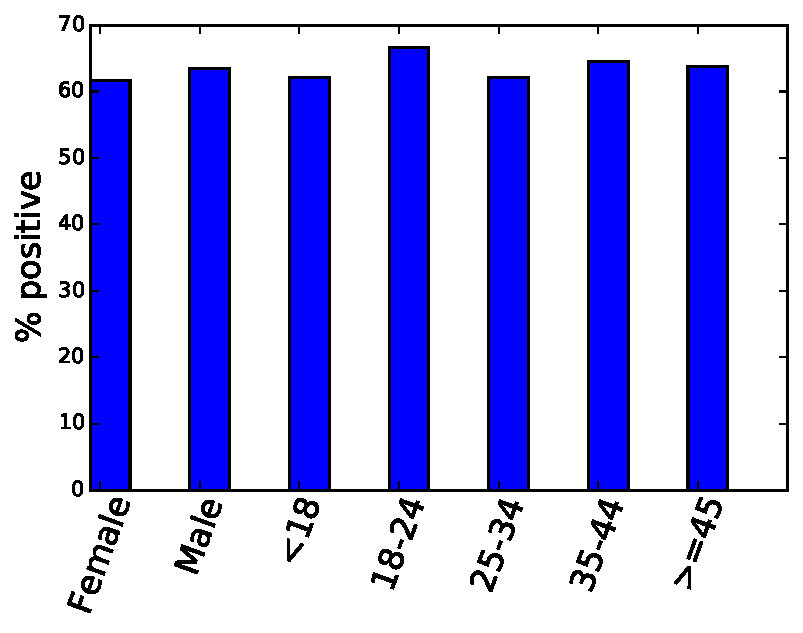
\includegraphics[width=\columnwidth]{nb/pct_pos.pdf}  % 111.png}
\caption{Percent of non-neutral tweets from each group classified as expressing positive sentiment towards e-cigarettes.\label{f.pct_pos}}
\centering
\end{figure}

\begin{figure*}[t]
  \caption{Tweets by gender and sentiment.}
  \begin{subfigure}{\columnwidth}
    \centering
    \caption{Tweets by gender. \label{f.gender}}
    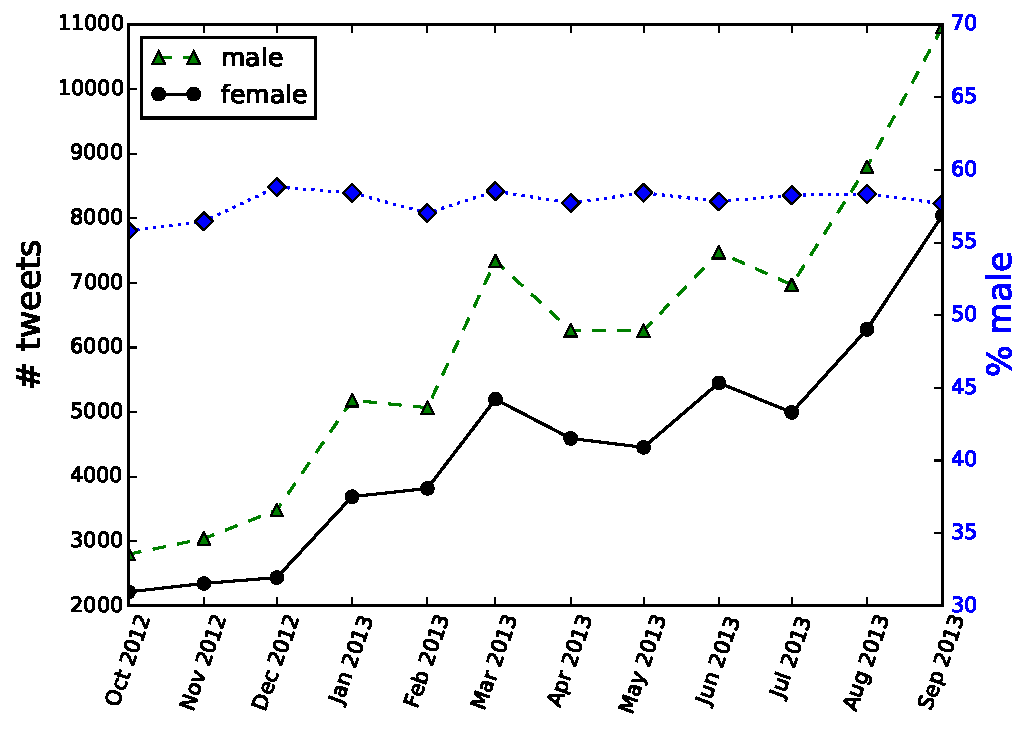
\includegraphics[width=\columnwidth]{nb/gender.pdf}
  \end{subfigure}
  \begin{subfigure}{.93\columnwidth}
    \centering
    \caption{Tweets by gender by sentiment.  \label{f.gender.sentiment}}
    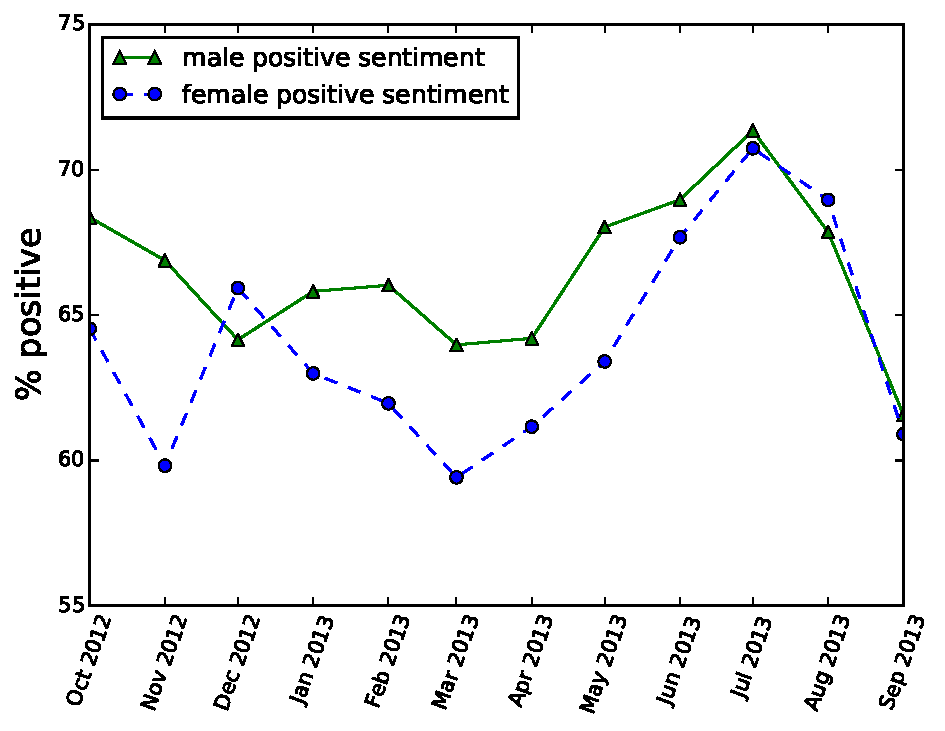
\includegraphics[width=\columnwidth]{nb/gender_sentiment.pdf}
  \end{subfigure}
\end{figure*}


\begin{figure*}[t]
  \caption{Tweets by age and sentiment.}
  \begin{subfigure}{.9\columnwidth}
    \centering
    \caption{Tweets by age. \label{f.age}}
    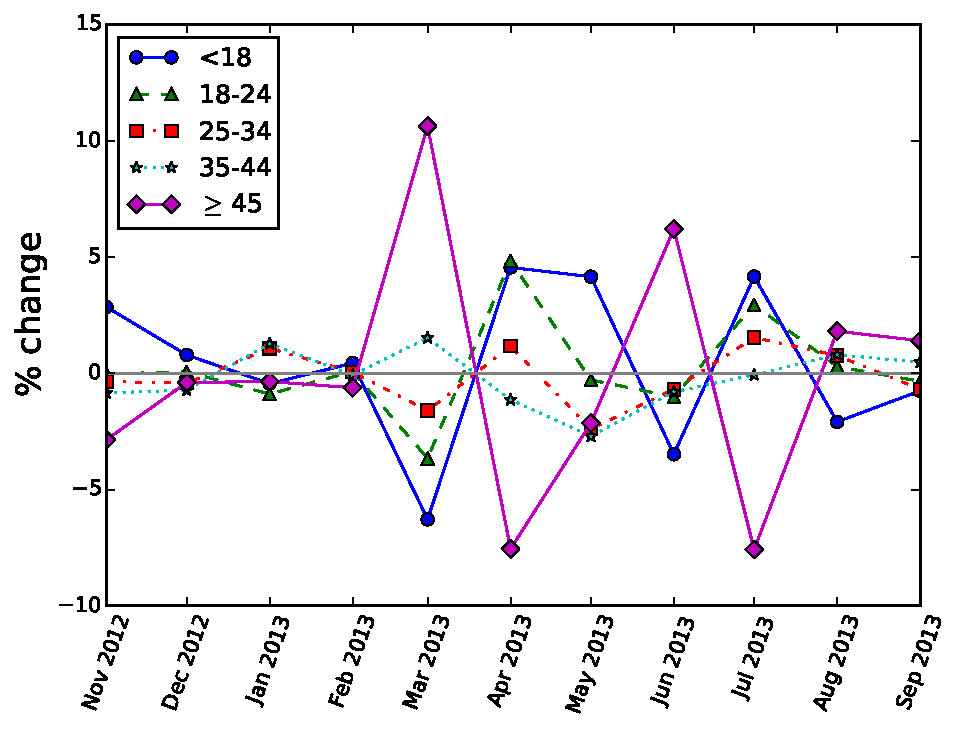
\includegraphics[width=\columnwidth]{nb/ages.pdf}
  \end{subfigure}
  \hspace{.5in}
  \begin{subfigure}{\columnwidth}
    \centering
    \caption{Tweets by age by sentiment.\label{f.age.sentiment}}
    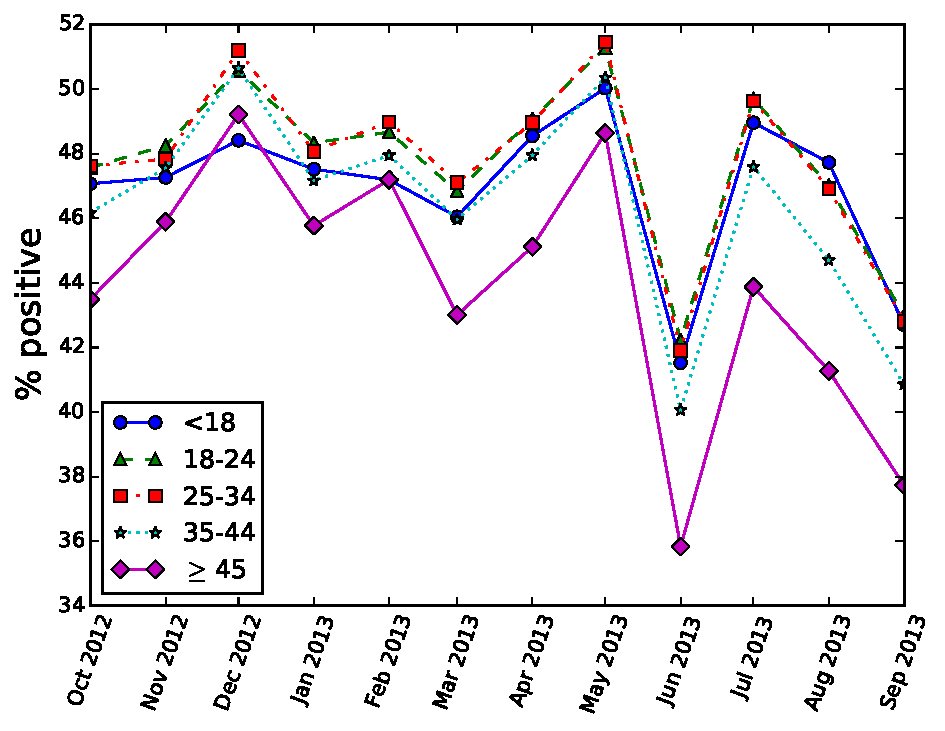
\includegraphics[width=\columnwidth]{nb/age_sentiment.pdf}
  \end{subfigure}
\end{figure*}



\begin{table*}[t]
\centering
\caption{Significant terms by category. \label{t.coef_demo}}
\label{tab:terms}
\begin{tabular}{|r|p{14cm}| }
\hline
{\bf Positive sentiment} & my, i, got, ecig, need, love, e-cig, me, i'm, cig, lost, mom, want, vaping, bought, dad, broke, so, just, get\\
{\bf Negative sentiment} & class, smoking, an, you, in, kid, cool, electric, people, guy, look, smoke, he, you're, stupid, if, fuck, dude, cigarette, are\\
\hline
{\bf Female} & cigarette, my, her, electric, mom, dad, smoking, me, amp, electronic, an, class, omg, \#giveaway, so, x, his, boyfriend, i, onew\\
{\bf Male} & vaping, green, e-cigs, bro, blu, pope, e-cigarettes, @blucigs, ban, \#vape, @youtube, stephen, the, game, pussy, new, a, any, vapers, gay\\
\hline
{\bf <18} & electric, cig, class, an, cigarette, e, lol, just, mom, cool, those, guy, haha, was, hookah, mask, elaborate, dad, shit, my\\
{\bf 18-24} & electric, cigarette, those, lol, cig, class, her, fait, electronique, blu, hookah, got, smh, cutting, laugh, quand, feel, me, mom, commercial\\
{\bf 25-34} & an, cigarette, electric, cig, class, my, just, those, i, bought, guy, so, her, girl, his, mom, kid, dad, me, cigs\\
{\bf 35-44} & cigarette, \#gotitfree, electric, those, blu, i, cigs, just, cig, bought, an, these, was, lol, electronic, luck, her, it, what, smoking\\
{\bf $\geq$ 45} & electric, thuis, markten, cigarette, alle, van, hq, those, blu, via, e-smoking, e-cigarette, elaborate, @lord\_sugar, mask, just, cigs, mistic, reviews, was\\
\hline
{\bf 2012-10} & electric, cigarette, electronic, cigarettes, green, free, alternative, trial, class, those, obtain, an, during, enjoys, liked, looks, obama, photo, stephen, lol\\
{\bf 2012-11} & election, cigarette, electric, mask, elaborate, electronic, kristen, traditional, device, rob, halo, na, brand, knee, touching, kit, cigarettes, lol, was, class\\
{\bf 2012-12} & christmas, electric, elaborate, cigarette, mask, electronic, @overlymanlymann, na, ko, addiction, advertising, ako, ny, ng, cigarettes, hq, allowed, calif, report, those\\
{\bf 2013-01} & prevent, electric, accessories, regulating, rolling, sale, cigarette, banning, electronic, na, fda, continue, ng, ko, launch, tv, those, haha, cigarettes, ni\\
{\bf 2013-02} & amg, miracle, menace, boat, racing, electric, drive, cigarette, elaborate, mask, prevent, class, decision, 99/99, crave, continues, electronic, including, opinion, @e\_swisher\\
{\bf 2013-03} & onew, green, utah, cigarette, gallagher, noel, muse, pope, drummer, caught, moves, criticises, electronic, electric, \#gotitfree, risks, smoke, mistic, tax, an\\
{\bf 2013-04} & courtney, f-bomb, drops, ad, love, @simoncowell, electric, njoy, \#gotitfree, inside, bring, commercial, cigarette, blu, class, an, lol, those, i, watch\\
{\bf 2013-05} & @lord\_sugar, france, la, electronique, les, governo, logic, places, electric, ecig, une, my, an, public, c'est, electrique, lol, il, mais, cigarette\\
{\bf 2013-06} & e-smoking, package, restrictions, incredible, britain, rise, medicines, include, kits, medicine, website, parker, face, markten, experience, easy, perfect, alle, thuis, reynolds\\
{\bf 2013-07} & markten, van, alle, thuis, vuse, vaporizer, \#uk, e-cig, ook, my, op, hookah, ecig, tweets, being, i, ik, regulation, blu, me\\
{\bf 2013-08} & promise, markten, companies, benowitz, neal, thuis, echo, van, cigs, heyday, alle, york, e, stadium, literally, merthyr, professor, never, bloomberg's, ook\\
{\bf 2013-09} & doubles, among, patches, students, teens, cdc, e-cigarettes, use, kids, effective, flames, 9-foot, survey, shows, markten, middle, u.s, teach, e-cigarette, study\\

\hline
\end{tabular}
\end{table*}


\subsection{Gender}

Overall, we identified 73,647 male and 53,528 female tweets from the filtered
set of 455K tweets. We were unable to identify gender for the remaining
tweets; many users leave the name field blank or enter a fake
name. Figure~\ref{f.gender} plots the gender distribution by month, and
Figure~\ref{f.gender.sentiment} plots the percentage of non-neutral tweets
labeled as positive by gender.

Males consistently tweets about cigarettes more than females for all
months. Moreover, male sentiment is typically more positive than female
sentiment, and the sentiment trends between the two groups are mostly
comparable. An exception is December 2012, in which male sentiment decreases,
but female sentiment increases, surpassing male sentiment. Examining positive,
female tweets in December, we observe a number of tweets indicating attempts
to get family members to quit smoking using e-cigs, e.g., ``{\sl Ima buy my
  dad an electronic cigarette for Christmas, no more tobacco pal}''; ``{\sl
  About to make my dad's day with an early Christmas present. I got him an
  E-Cig so he'll quit smoking.}''; ``{\sl My mom got an E-smoke for
  christmas. Anything to get her to quit}.'' There are also a smaller number
of tweets indicating parents smoking e-cigs with their children, e.g., ``{\sl
  Smoking an e-cig with my dad \#uh}.''

As in the previous section, we computed Chi-Squared statistics for each feature
to identify the top terms correlating with each gender. The second and third
rows of Table~\ref{t.coef_demo} further confirm that females are more likely
to discuss e-cigs in reference to other family members, whereas males are more
likely to discuss their own e-cigs (``my'') as well as to use profanities to
insult e-cig users. Furthermore, the appearance of ``class'' on the female
list suggests that many of the negative tweets about smoking in class (see the
previous section) are authored by female users.

\subsection{Age}
Unlike for gender, for age we compute a distribution over brackets for each
user. When we compute the average of these distributions for all users, we get
the following estimated age distribution: under 18: 32\%, 18-24: 13\%, 25-34:
16\%, 35-44: 14\% and 45+: 25\%. Due to well-known sample bias in Twitter
users, we expect that this result over-estimates the prevalence of the very
young and the very old (as in \citenoun{paval2015confounds}). Thus, we focus
on the month-by-month differences in these distributions. Figure~\ref{f.age}
shows the percent change for each bracket in each month.

The large spike in 45+ users in March 2013 appears to be due in part to a
word-of-mouth marketing campaign promoting e-cigs; \#gotitfree and \#giveaway
are used disproportionately more by 45+ users in this month. The spike in
young users in April and May appears to be in part due to a viral video of the
musician Courtney Love promoting NJOY brand e-cigs in a commercial containing
profanity. This was disproportionately shared and discussed by young users.

To visualize the relation between age and sentiment, we assigned each user the most likely age bracket based on their estimated distribution. We then computed the percentage of positive sentiment tweets by age bracket. Figure~\ref{f.age.sentiment} plots these values by month. The spike in positive sentiment for young users in June-August 2013 again appears to be due in part to the drop in tweets about smoking in class, as discussed in Section~\ref{s.sentiment_results}.

Table~\ref{t.coef_demo} also shows the terms with the strongest correlation to each age bracket. Intuitively, the term ``class'' tends to be indicative of younger users, as are references to ``mom'' and ``dad.'' Older users tend to use fewer abbreviations (e.g., ``electronic cigarettes'' vs. ``ecigs''); they also appear to be more likely to participate in word-of-mouth marketing campaigns (``\#gotitfree''). It is possible that these older users may in fact be part of a coordinated ``astroturf'' campaign on behalf of e-cig companies, though further analysis is required to verify this.

Finally, Figure~\ref{f.pct_pos} shows the percentage of non-neutral tweets from each
demographic category that are labeled as positive. We observe somewhat more
positive sentiment among males, and the highest sentiment among 18-24 year
olds.  The higher sentiment of this age group is in line with some survey
results of e-cig usage. A meta-analysis found ever-use highest among young
adults (20-28 year olds)~\cite{chapman2014cigarette}; while
\citenoun{regan2013electronic} found 18-24 year olds to have the highest rate
of ever-use. \citenoun{pearson2012cigarette} also find higher usage among
males.



\section{Conclusions and Future Work}
\label{s.conclusion}

In this paper we have quantified trends in e-cig messages posted to
Twitter. Overall, the volume of tweets mentioning e-cig terms has grown
five-fold from October 2012 to September 2013. A sentiment analysis classifier
indicates that males and young users are more likely to post positive tweets,
which either support e-cigs or mention their usage. The open-ended nature of
the data provides opportunity for additional analysis that may be difficult
with traditional surveys; for example, we find many users posting negative
comments about fellow students smoking in class; many female users mentioning
buying e-cigs to help family members stop smoking; and older users
participating in promotional campaigns. Such observations may suggest avenues
for future research and interventions.

There are a number of limitations and difficulties using such a noisy data
source. While some trends match the conclusions of traditional surveys (e.g.,
younger, male users were most likely to post positive messages), the tweet
volume is often influenced by rare events, such as a viral commercial
(Courtney Love) or photograph (Onew smoking an e-cig). These events lead to a
spike in messages that may not reflect true sentiment toward e-cigs. While we
have taken steps to mitigate these (e.g., removing duplicate tweets), new
methods are required to disentangle ``genuine'' tweets versus ``pop culture''
tweets. Additionally, it may be fruitful to investigate ways to measure the
long-term impact of such one-time events; for example, did the Courtney Love
video lead to an overall increase in e-cig awareness?

Additionally, while our analysis used a year of data, a multi-year study may
be required to remove some of the observed cyclical effects (e.g., the
academic year and end-of-year holidays appear to influence observed
sentiment). Finally, we have used only first name statistics to infer age and
gender. In future work, we will consider more sophisticated approaches to
infer a wider range of attributes with higher precision and
recall~\cite{culotta2015predicting}.


\section{Acknowledgments}
This work was supported in part by the National Science Foundation under grant
\#IIS-1526674.  Any opinions, findings and conclusions or recommendations
expressed in this material are the authors' and do not necessarily reflect
those of the sponsor.

\bibliographystyle{abbrvnat}
\bibliography{report} %
% You must have a proper ".bib" file
%  and remember to run:
% latex bibtex latex latex
% to resolve all references
%
% ACM needs 'a single self-contained file'!
%
%\balancecolumns % GM June 2007
% That's all folks!
\end{document}
